\newpage
\appendix

\chapter{Exo-FMS}\label{ap:exo-fms}


% 0 -- LEAD-IN PARAGRAPHS

%START ELEMENT
Three-dimensional simulations are an important tool for understanding atmospheric dynamics and climate.

A General Circulation Model (GCM)


%FRAMING TEXT
This chapter describes my work on the GCM Exo-FMS, and discusses the specific needs and issues of the atmospheres that I simulated with it.

%SIGNPOSTS
I will discuss the dynamical core and grid of the model

%SUMMARISE CONCLUSIONS
This chapter does not include much scientific investigation, but I will try to show that an exoplanet GCM is not a fanciful attempt to recreate an unknowable planet, but can be used carefully alongside basic theories and real observations to understand processes that are only apparent in a full 3D representation of the planetary atmosphere. I will also argue that XX.

%SECTION 0 -- MODEL STRUCTURE
\section{Model Structure}

%SUBSECTION -- FMS
\subsection*{GFDL-FMS}

Exo-FMS is based on the cubed-sphere dynamical core of the GFDL FMS.


%SUBSECTION -- GITHUB
\subsection*{Github Repository}

It was very important that Exo-FMS should be openly available. I manage its Github repository and wiki.


%SUBSECTION -- NEW INTERFACE
\subsection*{ExoFMS Interface}

Exo-FMS is meant to make the fewest modifications to the original FMS structure and cubed-sphere dynamical core as possible. To this end, I wrote a single interface to couple the dynamical core to our physics modules (radiative transfer, convection etc.).



%SECTION 1 -- DYNAMICS
\section{Dynamics}

The dynamical core of the GFDL-FMS solves the primitive equations.

%SUBSECTION -- LAT-LON

For the work in Chapter \ref{ch:linking-climate-55cnce}, I used a dynamical core with a latitude-longitude grid. This grid was divided up by latitude, with each processors handling a certain number of latitude bands (three by default).

We found that the latitude-longitude grid did not deal well with instabilities at the poles of our simulations, particularly the very hot, tidally locked atmospheres under investigation. On a latitude-longitude grid, the cells get smaller and less stable towards the pole, and schemes are required to deal with cross-polar transport and instabilities. This led to the model unpredictably crashing without a particular cause.

%SUBSECTION -- CUBED-SPHERE

To solve this problem, I updated the model to use a cubed-sphere grid.

A cubed-sphere grid is X.

As the version of the overall FMS system was newer for the new cubed-sphere dynamical core, it was simpler to just start again and treat it as a new model.

%SECTION CONCLUSIONS


%SECTION 2 --RADIATIVE TRANSFER
\section{Radiative Transfer}

%SUBSECTION -- GREY-GAS

I used a semi-grey radiative transfer scheme.

%SUBSECTION -- SOCRATES

%SECTION CONCLUSIONS


%SECTION 3 -- CLOUDS
\section{Cloud Microphysics}

%SUBSECTION -- DIHRT

%SUBSECTION -- INTERFACE TO SOCRATES

%SECTION CONCLUSIONS


%SECTION 4 -- PLANETS
\section{Example Planets}

%SUBSECTION -- TEMPERATE TERRESTRIAL PLANETS
\subsection{Temperate Terrestrial Planets}


%SUBSECTION -- LAVA PLANETS
\subsection{Lava Planets}


%SUBSECTION -- GAS PLANETS
\subsection{Gas Planets}


%SECTION CONCLUSIONS



%CONCLUSIONS

%RESTATE SECTION CONCLUSIONS

%OPEN OUT CONCLUSIONS

\chapter{GFDL-SDC}\label{ap:gfdl-sdc}

The non-linear shallow-water simulations in Chapter X were run using the Geophysical Fluid Dynamics Laboratory Spectral Dynamical Core (GFDL-SDC).

\section{Model Details}

The GFDL-SDC uses a spectral solver.

\section{Simulation Details}

I used a shallow-water variant of the GFDL-SDC, with a single layer following the shallow-water equations:

The tests in Figure X were forced by a relaxation to the height field X, the same as the linear theory in Chapter X.

The tests in Figure X also had a zonal acceleration applied with the form X, the same as the tests of the linear theory in Chapter X.




\chapter{Pseudo-Spectral Methods}\label{ap:ps-methods}


In this appendix, we discuss how we solved the linearized shallow-water equations using a pseudo-spectral collocation method \citep{boyd2000spectral}. Defining a linear ordinary differential equation or system of equations:

\begin{equation}
  L u = q
\end{equation}

$L$ is a differential operator acting on the variable $u$, and $q$ is the forcing or eigenvalue term. The solution is written as a sum of a series of basis functions:

\begin{equation}\label{eqn:pseudospectral_sum}
  u(x) = \Sigma a_{n} \psi_{n}(x)
\end{equation}

For a system of equations rather than a single equation, $L$ is a matrix and $u$ and $q$ are vectors. We impose the condition that the differential equation is satisfied at $N$ ``collocation points'', the positions of which depend on the set of basis functions.

This is equivalent to specifying that the ``residual'' -- the difference between the exact solution and the pseudo-spectral series solution -- is zero at these points. This provides $N$ equations to solve for the $N$ unknowns $a_{n}$, which gives the matrix equation:

\begin{equation}\label{eqn:ps_matrix}
  \textbf{H} \textbf{a} = \textbf{f}
\end{equation}

\section{Solving Equations}


\subsection*{Solving One Equation}

 \citet{boyd1978shearI} solves the linearized shallow-water equations, by reducing them to a single equation for a single variable, and applying the pseudo-spectral method. In this paper, we solve the entire system of shallow-water equations at once with the method in Appendix \ref{sec:app-systems}, but explain the method for a single equation here as it naturally leads to the second method \citep{boyd2000spectral}.

The matrix elements $H_{ij}$ in equation \ref{eqn:ps_matrix} are evaluated using the operator $L$ at the collocation points $x_{i}$ and for every mode $\phi_{j}$, and the vector elements $f_{i}$ are the terms $q$ evaluated at the collocation points $x_{i}$:

\begin{equation}\label{eqn:ps_H}
  H_{ij} = L \phi_{j}(x_{i})
\end{equation}

\begin{equation}
  f_{i} = q(x_{i})
\end{equation}


This is then solved using a standard linear algebra routine to find $a_{n}$, and the solution $u(x)$ is reconstructed using Equation \ref{eqn:pseudospectral_sum}.


\subsection*{Solving Systems of Equations}\label{sec:app-systems}

The pseudo-spectral method can also be applied to systems of linear ordinary differential equations. For a system of forced, time-independent equations:

\begin{equation}
  \textbf{L} \textbf{u} = \textbf{q}
\end{equation}


The condition that the differential equation is satisfied at the collocation points gives the equivalent matrix equation to Equation \ref{eqn:ps_matrix}:

\begin{equation}
  \textbf{H} \textbf{a} = \textbf{f}
\end{equation}

$\textbf{H}$ is an $M \times N$ square matrix with elements:

\begin{equation}
  H^{kl}_{ij} = L^{kl}\phi_{j}(x_{i})
\end{equation}

i.e. the operator $L^{kl}$ which acts on the $l$th variable in the $k$th equation, applied to the $j$th basis function and evaluated at the $i$th collocation point. $\textbf{f}$ is a vector made up of $N$ subvectors $f_{i}$, which are the forcing terms in each equation evaluated at each collocation point.

\begin{equation}
    \textbf{H} =
  \begin{pmatrix}
    \begin{pmatrix}
H_{ij} & \dots \\
\vdots & \ddots
    \end{pmatrix}^{kl} & \dots \\
  \vdots & \ddots
  \end{pmatrix}
  \begin{pmatrix}
    \begin{pmatrix}
    \alpha_{i} \\
    \vdots
    \end{pmatrix} \\
  \vdots
  \end{pmatrix}
  =
  \begin{pmatrix}
    \begin{pmatrix}
    f_{i} \\
    \vdots
    \end{pmatrix} \\
  \vdots
  \end{pmatrix}
\end{equation}

$\textbf{H}$ is the same as the matrix in Equation \ref{eqn:ps_H} with the elements $H_{ij}$ replaced by submatrices $H^{kl}_{ij}$. Solving this system returns the coefficients of the basis functions, and the solutions are:

\begin{equation}\label{eqn:ps-coeff-solutions}
 u(y) = \sum_{n=0}^{N} a_{n} \phi_{n}
; \quad
 v(y) = \sum_{n=0}^{N} b_{n} \phi_{n}
; \quad
 h(y) = \sum_{n=0}^{N} c_{n} \phi_{n}
\end{equation}


This gives a linear matrix equation with one solution corresponding to the coefficient vectors $a_{n}$, $b_{n}$, $c_{n}$ of the forced solution.

Without forcing, the shallow-water equations define an eigensystem where the eigenvalue is the frequency $\omega$.

\begin{equation}
  \textbf{L} \textbf{u} = \omega \textbf{P} \textbf{u}
\end{equation}

The pseudo-spectral equation is then:

\begin{equation}
  \textbf{H} \textbf{a} = \omega \textbf{R} \textbf{a}
\end{equation}

 $\textbf{R}$ is an $M \times N$ square matrix with elements:

\begin{equation}
  R^{kl}_{ij} = P^{kl}\phi_{j}(x_{i})
\end{equation}

i.e. the eigenvalue operator $P^{kl}$ acting on the $l$th variable in the $k$th equation, applied to the $j$th basis function and evaluated at the $i$th collocation point.

\begin{equation}
    \textbf{H} =
  \begin{pmatrix}
    \begin{pmatrix}
H_{ij} & \dots \\
\vdots & \ddots
    \end{pmatrix}^{kl} & \dots \\
  \vdots & \ddots
  \end{pmatrix}
  \begin{pmatrix}
    \begin{pmatrix}
    \alpha_{i} \\
    \vdots
    \end{pmatrix} \\
  \vdots
  \end{pmatrix}
  =
  \omega
  \begin{pmatrix}
    \begin{pmatrix}
R_{ij} & \dots \\
\vdots & \ddots
    \end{pmatrix}^{kl} & \dots \\
  \vdots & \ddots
  \end{pmatrix}
  \begin{pmatrix}
    \begin{pmatrix}
    \alpha_{i} \\
    \vdots
    \end{pmatrix} \\
  \vdots
  \end{pmatrix}
\end{equation}


This gives an eigenvalue matrix equation, with $N$ eigenvalues and eigenvectors, corresponding to the frequencies and coefficient vectors $a_{n}$, $b_{n}$, $c_{n}$ for each free mode. Not all $N$ modes must be physically realistic, so we identify the spurious modes by inspecting the eigenvalues for different values of $N$.


\begin{figure}
  \centering
  \begin{subfigure}[b]{0.4\textwidth}
    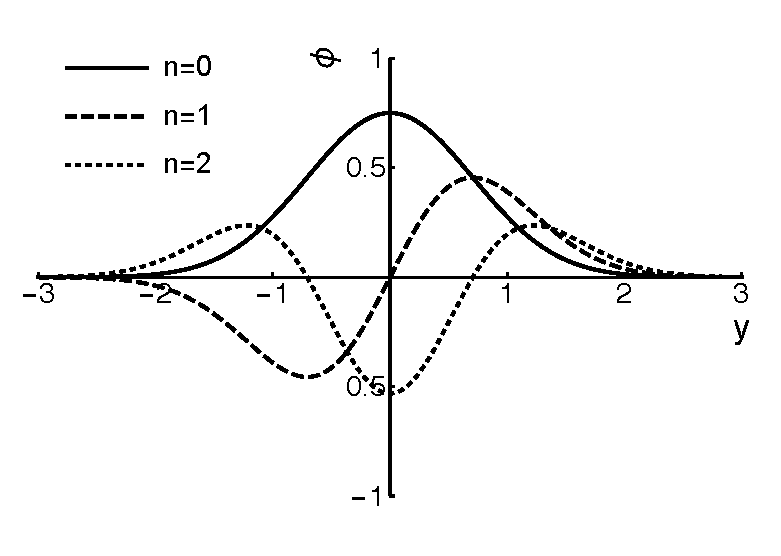
\includegraphics[width=\textwidth]{figures/appendices/hermite-functions.pdf}
    \caption{Parabolic Cylinder Functions}\label{fig:hermite-functions}
  \end{subfigure}
  %
  \begin{subfigure}[b]{0.4\textwidth}
    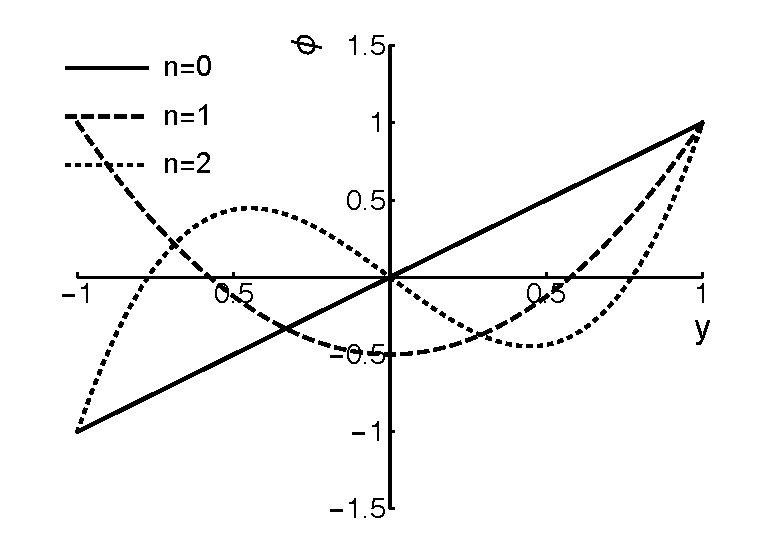
\includegraphics[width=\textwidth]{figures/appendices/legendre-polynomials.pdf}
    \caption{Legendre Polynomials.}\label{fig:legendre-polynomials}
  \end{subfigure}
\caption{Basis functions used in beta-plane and spherical coordinates.}\label{fig:basis-functions}
\end{figure}

\section{Example Solutions}


\subsection*{Beta-plane solutions}\label{sec:app-beta}

We use the \textbf{parabolic cylinder functions} $\psi_{n}(y)$ \citep{showman2011superrotation} as defined in Equation \ref{eqn:hermite-functions} as a basis set for the pseudo-spectral method on the beta-plane (Equation \ref{eqn:forced-sw}), as they are the exact free solutions of \citet{matsuno1966quasi} \citep{boyd2000spectral}.

Their collocation points are at their zeros (which are just the zeros of the Hermite polynomials $H_{n}$). Figure \ref{fig:hermite-functions} shows the first few \textbf{parabolic cylinder functions}.

\begin{equation}\label{eqn:hermite-functions}
  \psi_{n}(y) = e^{-y^{2} / 2} H_{n}(y)
\end{equation}

Figure \ref{fig:accuracy-hermite} shows the magnitude of the coefficients (Equation \ref{eqn:ps-coeff-solutions}) of the pseudo-spectral solution of the shallow-water equations linearized about a jet on a beta-plane (plotted in Figure \ref{fig:shear-2D}). The first plot shows that when the background jet flow is zero, only modes up to $n=2$ are non-zero. This is the analytic solution from \citet{matsuno1966quasi}, which the pseudo-spectral method identifies because we have used the free modes (the \textbf{parabolic cylinder functions}) as our basis functions.

For non-zero jet speed (corresponding to Figure \ref{fig:shear-2D}), the pseudo-spectral series solution does not terminate, but the coefficients for the 30th mode are about eight orders of magnitude smaller than the largest mode. The beta-plane solutions in this paper were all calculated with at least 30 modes.

\begin{figure}
    \centering
  \begin{subfigure}[b]{0.4\textwidth}
    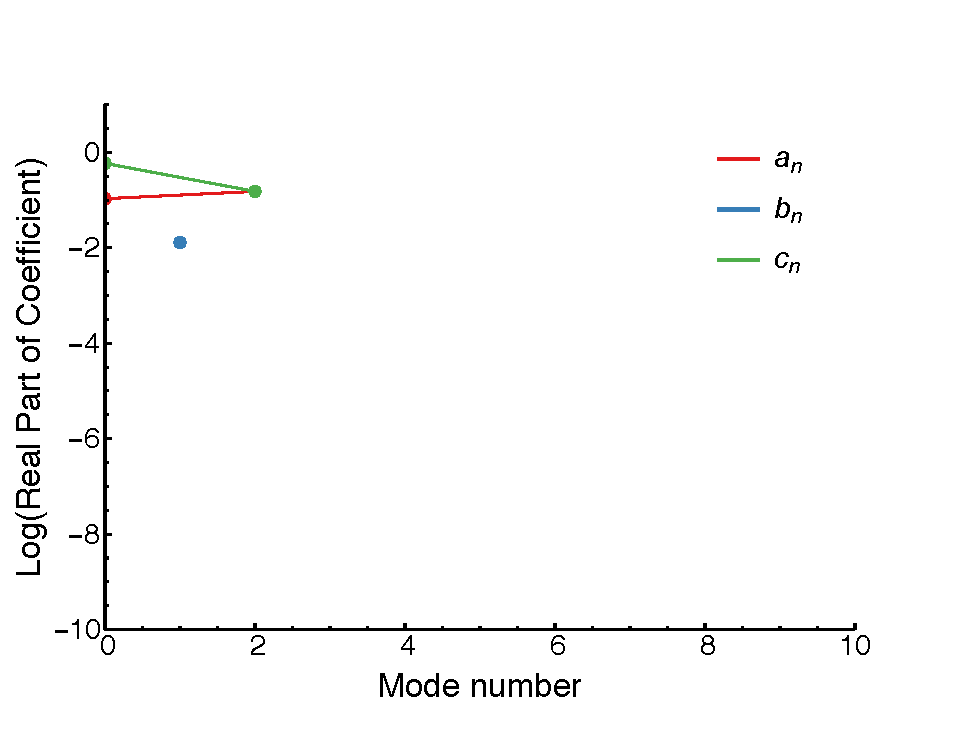
\includegraphics[width=\textwidth]{figures/appendices/zero-shear-hermite-accuracy.pdf}
    \caption{Coefficients for $\bar{U}(y)=0$.}
  \end{subfigure}
  %
  \begin{subfigure}[b]{0.4\textwidth}
    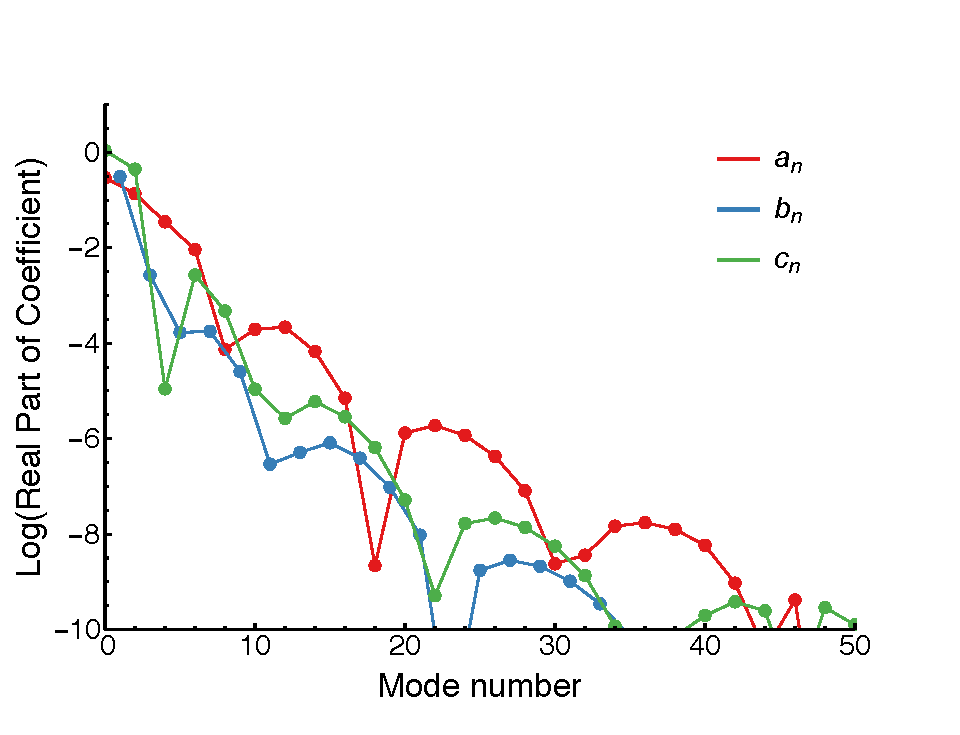
\includegraphics[width=\textwidth]{figures/appendices/shear-hermite-accuracy.pdf}
    \caption{Coefficients for $\bar{U}(y)=\exp(-y^{2}/2)$.}
  \end{subfigure}
\caption{Coefficients of the pseudo-spectral solution on the beta-plane coordinates with and without a background jet (the plots in Figure \ref{fig:shear-2D}). The method identifies the exact solution in the first case, and converges rapidly to an accurate solution in the second case. }\label{fig:accuracy-hermite}
\end{figure}


\subsection*{Spherical solutions}\label{sec:app-spherical}

We use the Legendre polynomials as a basis set for the pseudo-spectral method in a spherical geometry (Equation \ref{eqn:sphere-sw-eqns}). Figure \ref{fig:legendre-polynomials} shows the first few Legendre polynomials. Our collocation points are the zeros of these functions.

As discussed in Section \ref{sec:sphere-solutions}, Equation \ref{eqn:sphere-sw-eqns} has a singularity at the the poles, which we avoided by using a rescaled height $\gamma$, where $\gamma = h / \cos\phi$ \citep{iga2005spherical}. We replaced $h$ with $\gamma \cos \phi$ in Equation \ref{eqn:sphere-sw-eqns}, solved as normal, then multiplied the solution for $\gamma$ by $\cos\phi$ to recover the solution for $h$.

Figure \ref{fig:accuracy-spherical} shows how rescaling the $h$ variable made the solutions converge much more quickly. In fact, the solutions without a rescaled $h$ variable never reached a smooth solution at the poles.


\begin{figure}
    \centering
  \begin{subfigure}[b]{0.4\textwidth}
    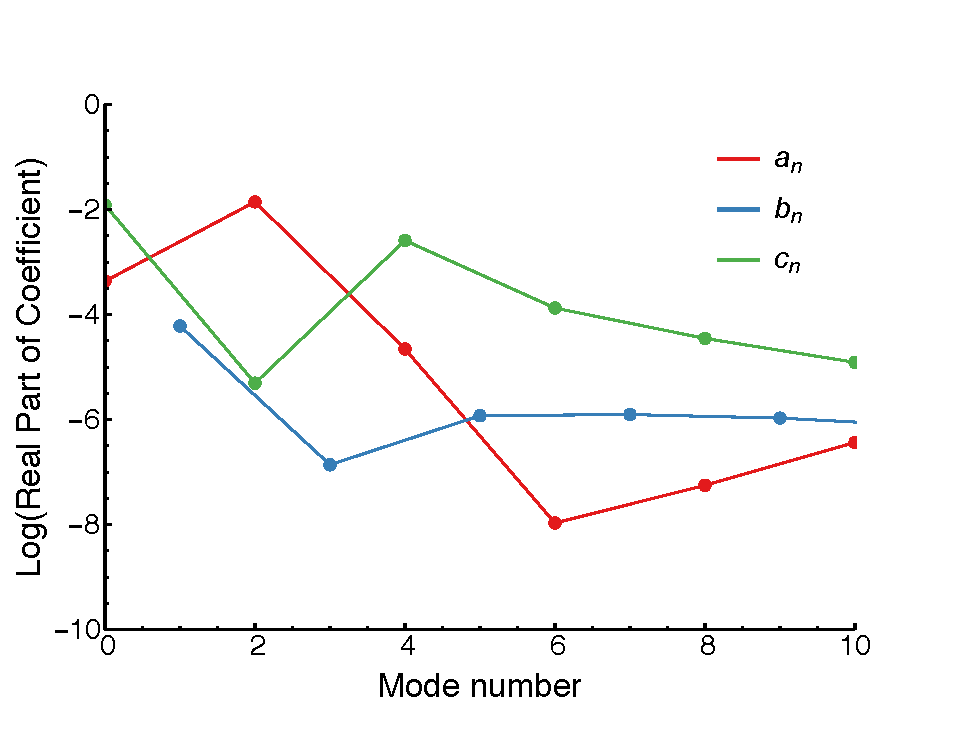
\includegraphics[width=\textwidth]{figures/appendices/sphere-accuracy-noscale.pdf}
    \caption{Coefficients calculated with height $h$.}
  \end{subfigure}
  %
  \begin{subfigure}[b]{0.4\textwidth}
    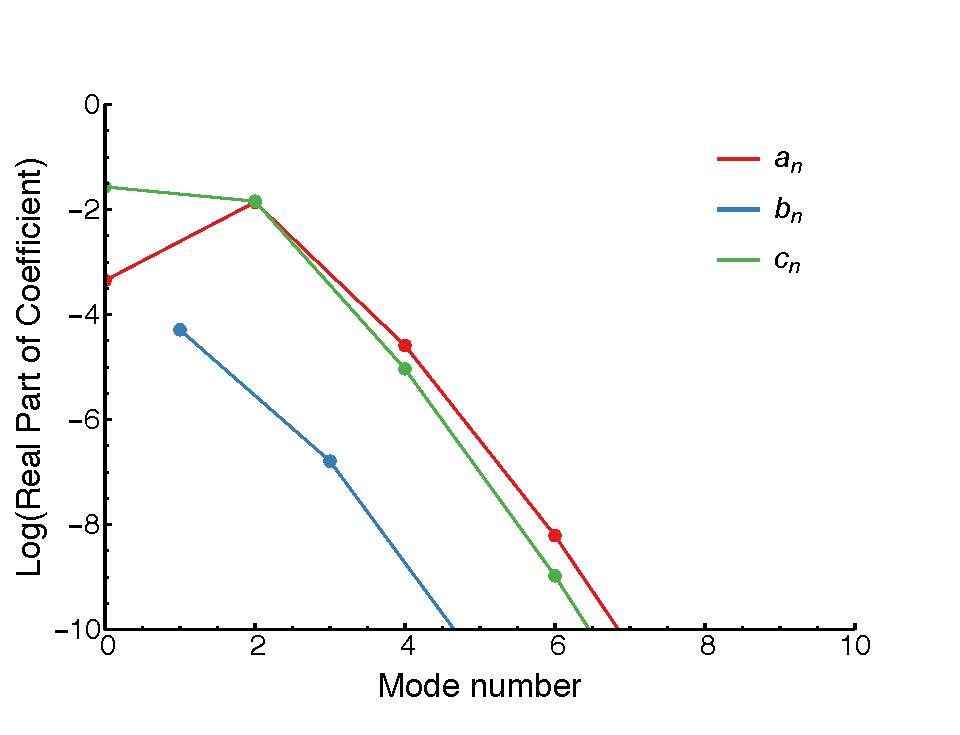
\includegraphics[width=\textwidth]{figures/appendices/sphere-accuracy-rescale.pdf}
    \caption{Coefficients calculated with rescaled height $\gamma = h / \cos\phi$.}
  \end{subfigure}
\caption{Coefficients of the pseudo-spectral solution in spherical coordinates (the first plot in Figure \ref{fig:spherical-tests}), with the height variable $h$ and the rescaled height $\gamma$. Rescaling the height makes the method converge to a smooth solution at the poles.}\label{fig:accuracy-spherical}
\end{figure}
